\subsection*{Explicación}
Para este ejercicio hice primero un MUX 2:1 para crear un MUX 4:1 que use para hacer un MUX 8:1 (que realmente no era necesario) para finalmente completar el MUX 16:1.
\subsection*{Código}
\faGithub \space
\href{https://github.com/warleon/Arch-lab1/tree/master/pregunta1}{https://github.com/warleon/Arch-lab1/tree/master/pregunta1}\\
make MUX\_16\_1
%\subsection*{Tabla de verdad}

%\subsection*{Mapa de Karnaugh}

%\subsection*{Ecuaciones booleanas}

\subsection*{Resultados}
\begin{figure}[h]
    \centering
    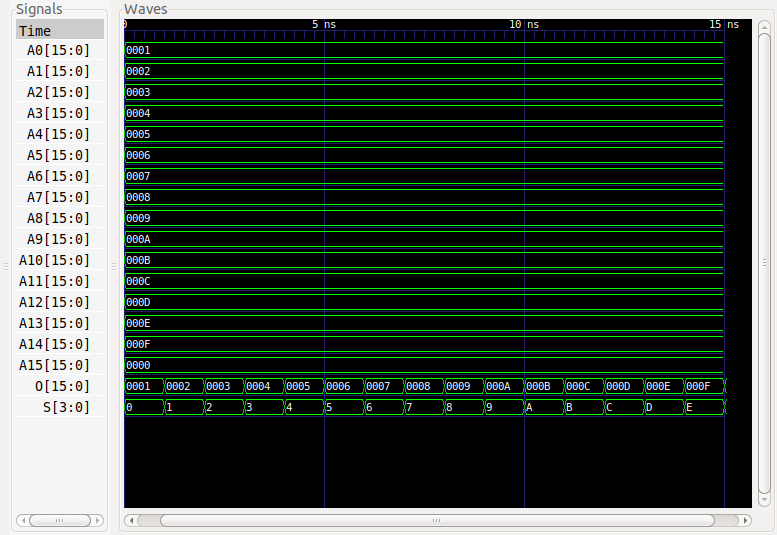
\includegraphics[scale=0.6]{fotos/resultados/arki-MUX_16_1.png}
    \caption{waves mux 16:1}
\end{figure}